\section{The Doppler Shift}

\begin{comment}
This lab is more of a worksheet than it is a lab.  But I've used versions of if in my 132 classes for a while, so I thought it was time to include it here in the lab manual for others as well.  --Matt Trawick, 6/2015

\end{comment}

\makelabheader %(Space for student name, etc., defined in master.tex)

\vspace{0.1in}
%\textbf{Objective} 
%


\textbf{Activity 1: Moving Source, Fixed Receiver}

\begin{center}
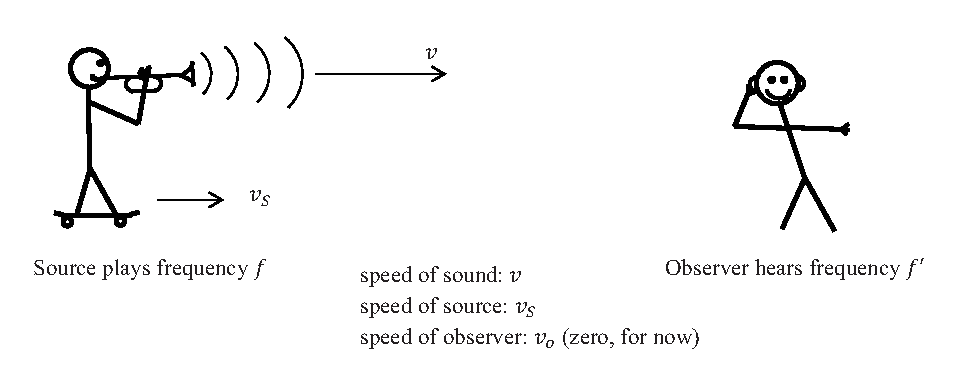
\includegraphics[width=0.75\textwidth]{doppler_shift/moving_source.eps}
\end{center}

Your friend (the ``source'') is playing the trumpet while riding towards you on a skateboard at speed $v_S$.  The first wavefront is emitted at time $t=0$.

(a) After one period $T$, how far has the first wavefront traveled?  (Answer in $v$, $f$.)
\vspace{1.0in}

(b) After one period $T$, how far has the source traveled? (Answer in $v_S$, $f$.)

\begin{wrapfigure}[1]{r}{0.33\textwidth}
\vspace{-1.5in}
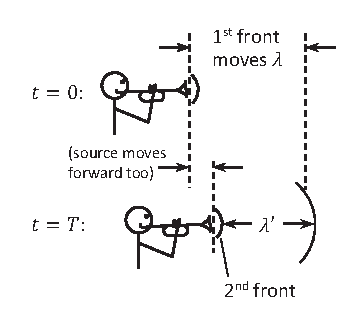
\includegraphics{doppler_shift/front_motion.eps}
\end{wrapfigure}

\vspace{1.0in}


At time $T$, the second wave front is emitted.

(c) What is the distance $\lambda'$ between the first two wave fronts?
\vspace{1.0in}

(d) The receiver sees a wave with speed $v$ and wavelength $\lambda'$.  What frequency $f'$ does the receiver hear? (Answer in $v, v_S, f$.)
\vspace{1.0in}

\pagebreak
\textbf{Activity 2: Moving Source and Moving Receiver}

\begin{center}
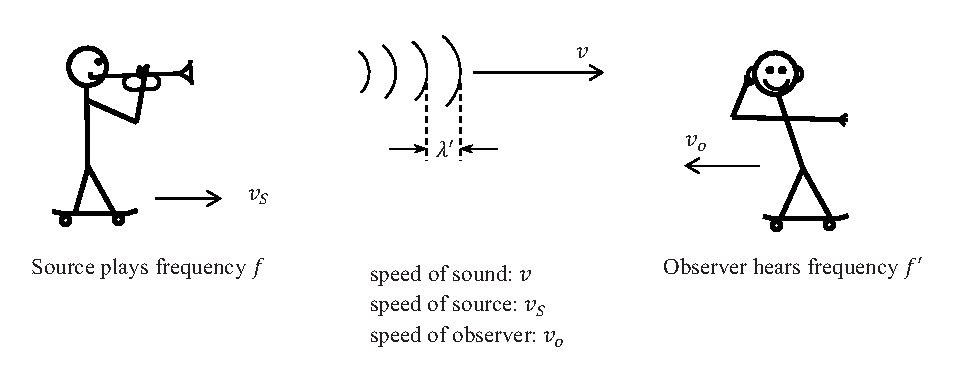
\includegraphics[width=0.75\textwidth]{doppler_shift/moving_observer.eps}
\end{center}

Now suppose that you are also moving towards the source with speed $v_R$.  

(e) What is the speed of the wave \textit{relative to the receiver}?  (That is, in the receiver reference frame, how fast do you see the wave coming at you?) 
\vspace{1.0in}

(f) What is the time $T'$ between the receiver hitting the first wavefront and the receiver hitting the second wavefront? (Answer in $\lambda', v, v_R$.)
\vspace{1.0in}

(g) Rewrite $T'$ in terms of $v, v_R, v_S$, and $f$, using your result from part (c).
\vspace{1.0in}

(h) So what frequency $f'$ does the receiver hear?
%\vspace{1.0in}

\vfill

Note our sign convention here:
\begin{align*}
\textrm{positive } v_R, v_S &\Longrightarrow \textrm{motion towards each other (``approaching'')} \\
\textrm{negative } v_R, v_S &\Longrightarrow \textrm{motion away from each other (``receding'')} 
\end{align*}
